\documentclass{article}
\usepackage[margin=1in]{geometry}
\usepackage{amsmath}
\usepackage{amssymb}
\usepackage{booktabs}
\usepackage{float}
\usepackage{graphicx}
\usepackage{hyperref}
\usepackage{pdfpages}
\usepackage{siunitx}
\usepackage{adjustbox}
\usepackage{cancel}
\usepackage{paracol}
\usepackage{placeins}

\usepackage{parskip}

\globalcounter{figure}
\counterwithin{equation}{section}

\title{Report}
\date{23 February 2026}
\author{Connor Emmons}

\begin{document}
\pagenumbering{gobble}
\maketitle
\vfill
\paragraph*{Notes}

\newpage
\pagenumbering{arabic}

\section{Initial Tests}

\section{Varying Number of Segments and Points}

\begin{figure}[H]
    \centering
    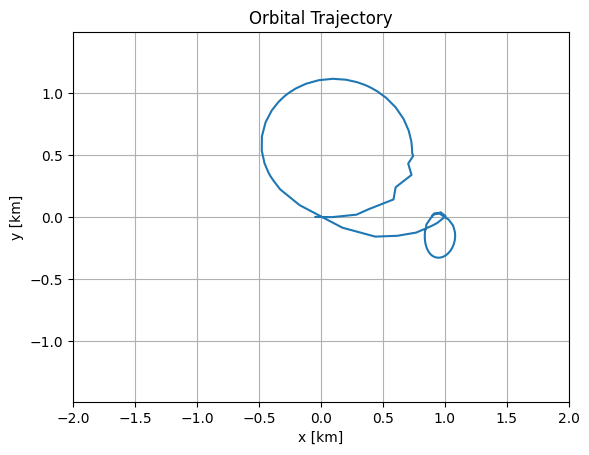
\includegraphics[width=0.9\columnwidth]{attempt1.png}
    \caption{Attempt 1}
    \label{fig: attempt1}
\end{figure}

\begin{figure}[H]
    \centering
    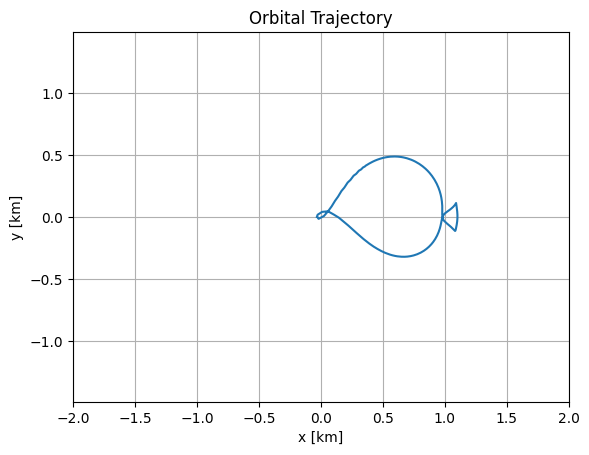
\includegraphics[width=0.9\columnwidth]{attempt2.png}
    \caption{Attempt 2}
    \label{fig: attempt2}
\end{figure}

\begin{figure}[H]
    \centering
    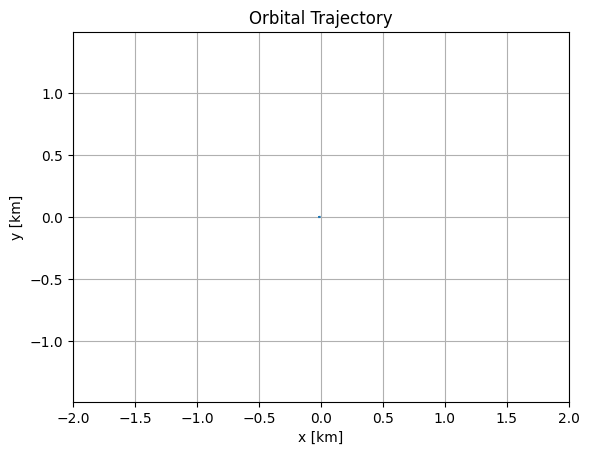
\includegraphics[width=0.9\columnwidth]{attempt3.png}
    \caption{Attempt 3}
    \label{fig: attempt3}
\end{figure}

\begin{figure}[H]
    \centering
    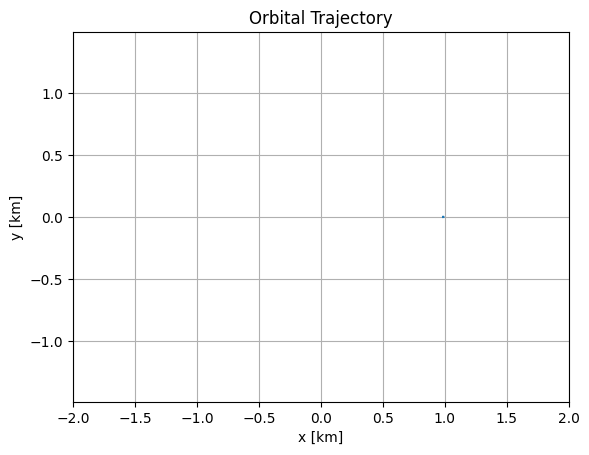
\includegraphics[width=0.9\columnwidth]{attempt4.png}
    \caption{Attempt 4}
    \label{fig: attempt4}
\end{figure}

\section{Added Lower Time Bound}

Realized that the final time was nowhere close, and with higher numbers of segments and points, only the trivial solution was found. Added lower time bound to fix.

\begin{figure}[H]
    \centering
    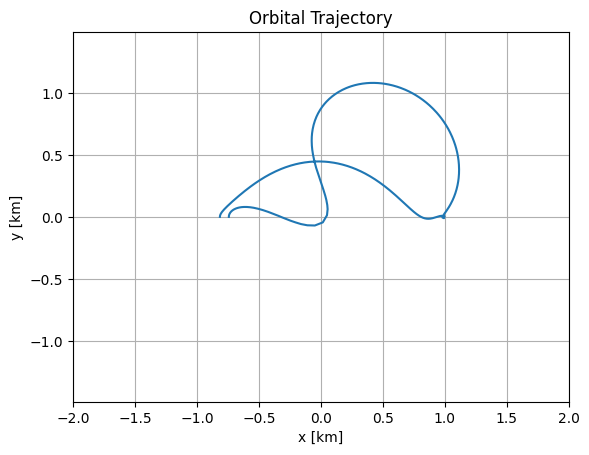
\includegraphics[width=0.9\columnwidth]{attempt5.png}
    \caption{Attempt 5}
    \label{fig: attempt5}
\end{figure}

\begin{figure}[H]
    \centering
    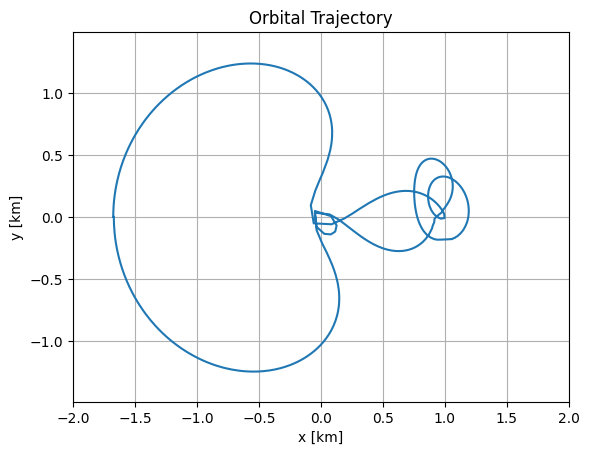
\includegraphics[width=0.9\columnwidth]{attempt6.png}
    \caption{Attempt 6}
    \label{fig: attempt6}
\end{figure}

\section{Added Upper Time Bound}
Added upper time bound and played with how tight the bounds were on the final time to the true period.

\begin{figure}[H]
    \centering
    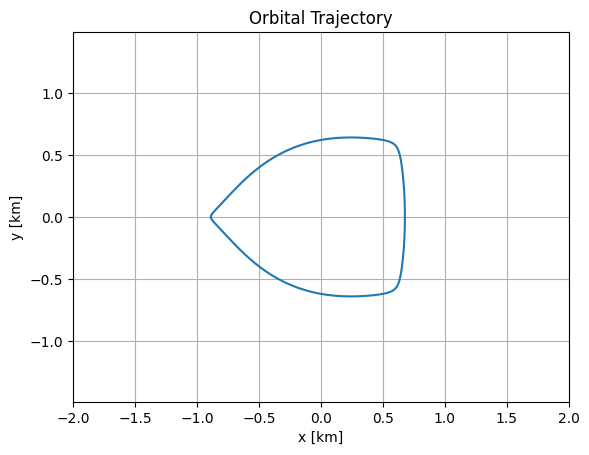
\includegraphics[width=0.9\columnwidth]{attempt7.png}
    \caption{Attempt 7}
    \label{fig: attempt7}
\end{figure}

Looks close, but period is $>$1 day off.

\begin{figure}[H]
    \centering
    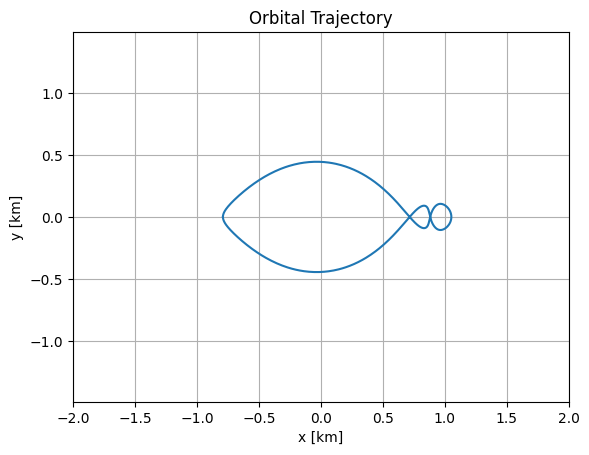
\includegraphics[width=0.9\columnwidth]{attempt8.png}
    \caption{Attempt 8}
    \label{fig: attempt8}
\end{figure}

\section{Fine Tuning of Segments, Points, and Tightness of Bounds}
Iterating on how bounds, segments, points, and tolerance. 

If segments/points are too high, the bad velocity guesses ruin the solution.

\begin{figure}[H]
    \centering
    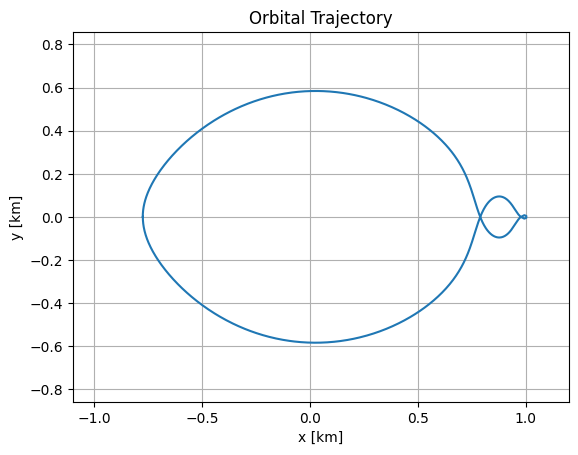
\includegraphics[width=0.9\columnwidth]{attempt9.png}
    \caption{Attempt 9}
    \label{fig: attempt9}
\end{figure}

\begin{figure}[H]
    \centering
    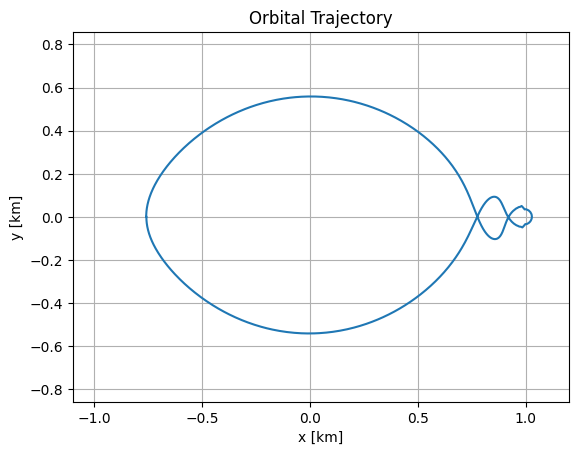
\includegraphics[width=0.9\columnwidth]{attempt10.png}
    \caption{Attempt 10}
    \label{fig: attempt10}
\end{figure}

\begin{figure}[H]
    \centering
    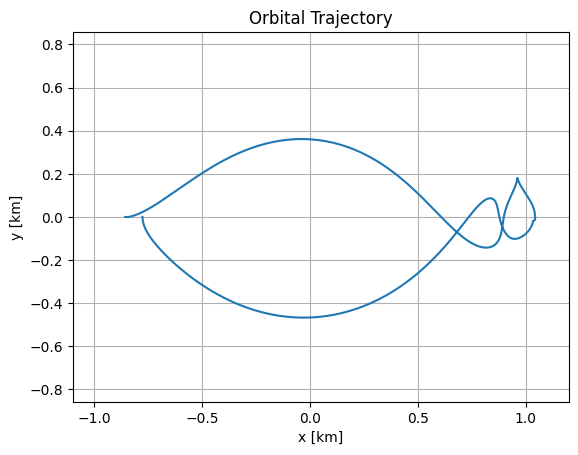
\includegraphics[width=0.9\columnwidth]{attempt11.png}
    \caption{Attempt 11}
    \label{fig: attempt11}
\end{figure}

\begin{figure}[H]
    \centering
    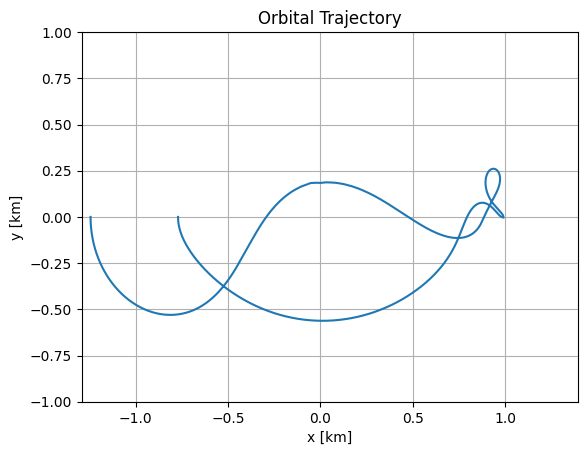
\includegraphics[width=0.9\columnwidth]{attempt12.png}
    \caption{Attempt 12}
    \label{fig: attempt12}
\end{figure}

\begin{figure}[H]
    \centering
    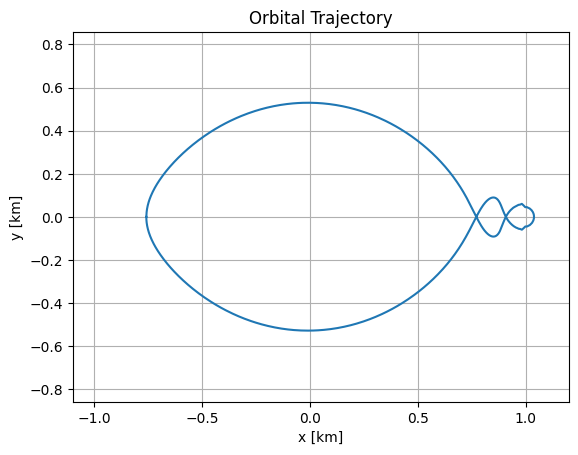
\includegraphics[width=0.9\columnwidth]{attempt13.png}
    \caption{Attempt 13}
    \label{fig: attempt13}
\end{figure}

\begin{figure}[H]
    \centering
    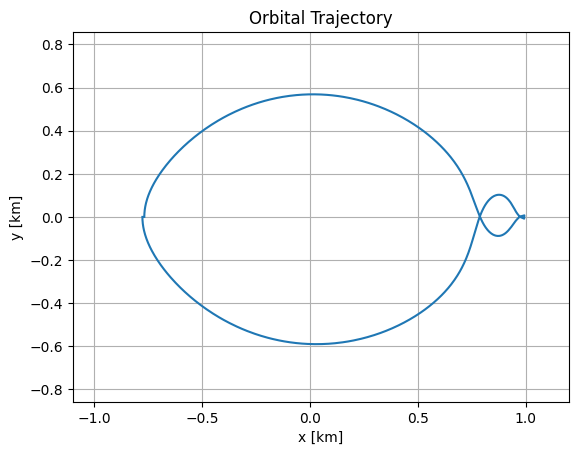
\includegraphics[width=0.9\columnwidth]{attempt14.png}
    \caption{Attempt 14}
    \label{fig: attempt14}
\end{figure}

\begin{figure}[H]
    \centering
    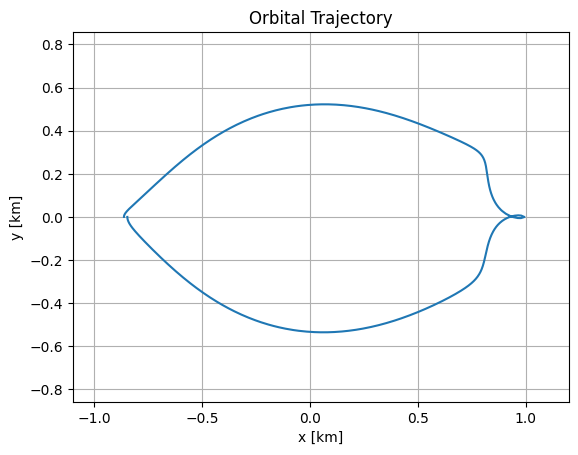
\includegraphics[width=0.9\columnwidth]{attempt15.png}
    \caption{Attempt 15}
    \label{fig: attempt15}
\end{figure}

Goldilocks zone of parameters to give a decent initial guess (~5 hours off of actual period)

\begin{figure}[H]
    \centering
    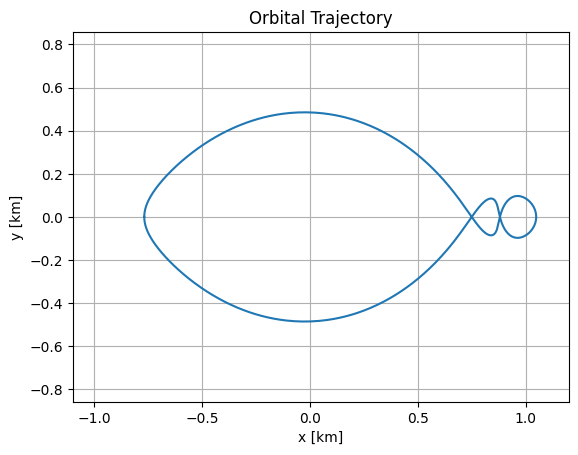
\includegraphics[width=0.9\columnwidth]{attempt16_good.png}
    \caption{Attempt 16 (Taken as initial guess for $k_1=k_2=1$ cyclers)}
    \label{fig: attempt16}
\end{figure}

\section{Further Refinement}

Kept decreasing the tolerance.

\begin{figure}[H]
    \centering
    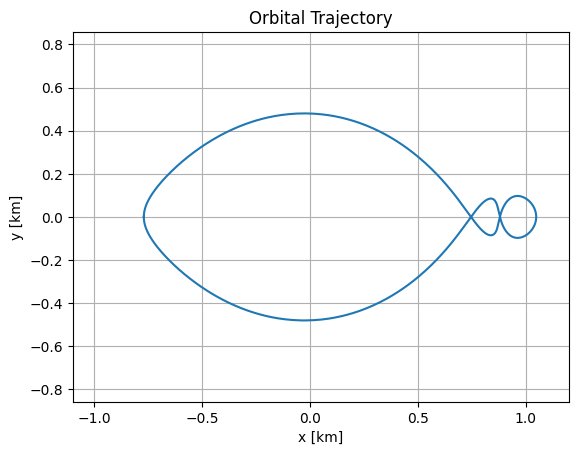
\includegraphics[width=0.9\columnwidth]{attempt17.png}
    \caption{Attempt 17}
    \label{fig: attempt17}
\end{figure}

\begin{figure}[H]
    \centering
    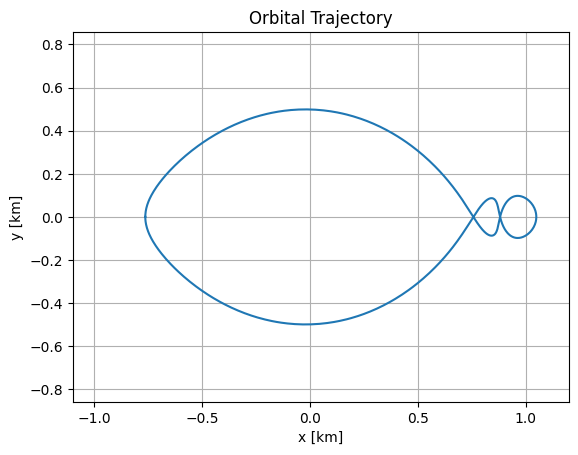
\includegraphics[width=0.9\columnwidth]{attempt18.png}
    \caption{Attempt 18}
    \label{fig: attempt18}
\end{figure}

Increasing segments and points from 30 to just 32 breaks the model.

\begin{figure}[H]
    \centering
    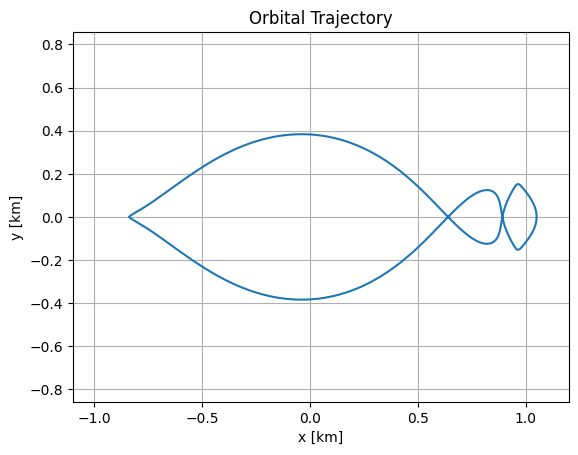
\includegraphics[width=0.9\columnwidth]{attempt19.png}
    \caption{Attempt 19}
    \label{fig: attempt19}
\end{figure}

\section{Final Initial Guess}

\begin{figure}[H]
    \centering
    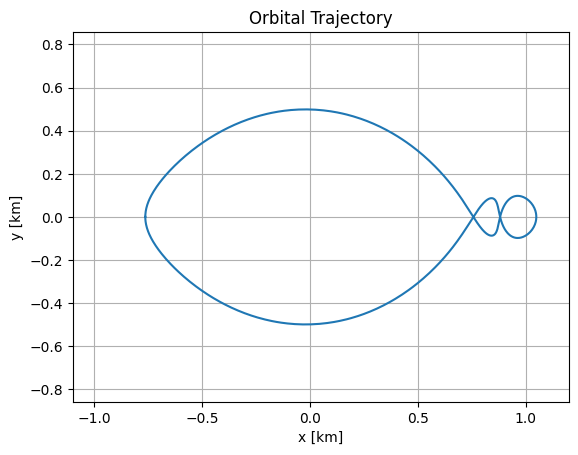
\includegraphics[width=0.9\columnwidth]{attempt20_better.png}
    \caption{Attempt 20 (best initial guess)}
    \label{fig: attempt20}
\end{figure}

\subsection{Parameters}

No objective function to minimize, set to just propogate the dynamics.

Orbital Parameter Guesses

\begin{itemize}
    \item $x_i = -0.767856324800$
    \item $C = 3.151175879508174$
    \item $y = \dot{x} = 0$
\end{itemize}

Bounds

\begin{itemize}
    \item $t_{i_{lower}} = t_{i_{upper}} = 0$
    \item $t_{f_{lower}} = 44.7538 - 1.5$ (further adjusted from days to time scale used in equations)
    \item $t_{f_{upper}} = 44.7538 + 1.5$
    \item discrete bounds = [0, 0, 0, 0]
    \item $\mathbf{x}_i[1:3] = \mathbf{x}_f[1:3] = [0, 0]$
\end{itemize}

Solver Parameters

\begin{itemize}
    \item segments = points = 30
    \item ipopt tol = 1e-20
\end{itemize}

\section{Final Initial Guess - Better}

Removing the last point at the end of the time window as a guess improved the results. New generated orbit is ~15 minutes off of stated period.

\begin{figure}[H]
    \centering
    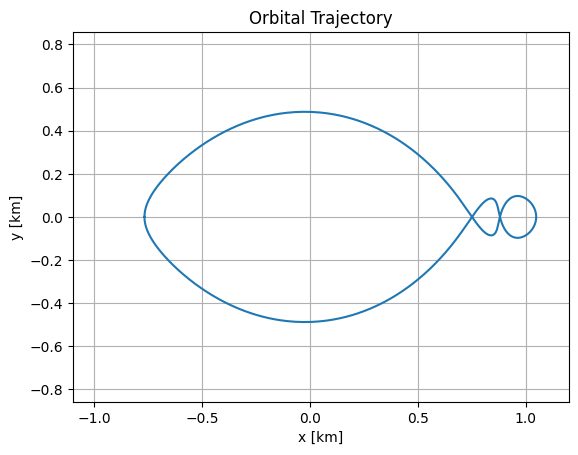
\includegraphics[width=0.9\columnwidth]{attempt21_best.png}
    \caption{Attempt 21 (best initial guess again)}
    \label{fig: attempt21}
\end{figure}

\begin{figure}[H]
    \centering
    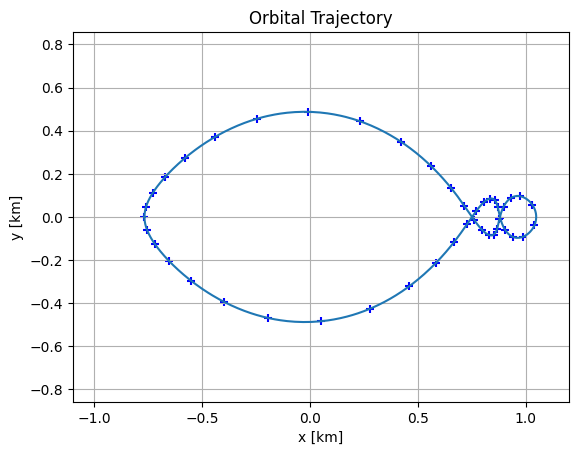
\includegraphics[width=0.9\columnwidth]{attempt21_days.png}
    \caption{Attempt 21 with day markers}
    \label{fig: attempt21 days}
\end{figure}

\subsection{Parameters}

No objective function to minimize, set to just propogate the dynamics.

Orbital Parameter Guesses

\begin{itemize}
    \item $x_i = -0.767856324800$
    \item $C = 3.151175879508174$
    \item $y = \dot{x} = 0$
\end{itemize}

Bounds

\begin{itemize}
    \item $t_{i_{lower}} = t_{i_{upper}} = 0$
    \item $t_{f_{lower}} = 44.7538 - 0.95$ (further adjusted from days to time scale used in equations)
    \item $t_{f_{upper}} = 44.7538 + 0.95$
    \item discrete bounds = [0, 0, 0, 0]
    \item $\mathbf{x}_i[1:3] = \mathbf{x}_f[1:3] = [0, 0]$
\end{itemize}

Solver Parameters

\begin{itemize}
    \item segments = points = 30
    \item ipopt tol = 1e-100
\end{itemize}

Error from stated period: 0.024\% (15.45 minutes)

\end{document}